\documentclass[border=4pt,12pt]{standalone}
% House style for redrawn exam diagrams (diagram-v4: 0.4pt lines, filled -latex arrows, fine dashes; stipple and hatching drawn as real dots/lines (no PDF/SVG patterns, so they render in every browser and at any scale); transparent background). Every figure \input's this.
\usepackage{amsmath,amssymb}
\usepackage{txfonts}
\usepackage{pdfrender,xcolor}
% \halo{text}: label on shading. The shading stops just around each letter's outline (a thin knock-out that follows the
% glyphs, like the papers' typesetting), never a box. Owner: "I don't want a box around the text".
\newcommand{\halo}[1]{\leavevmode\rlap{\pdfrender{TextRenderingMode=2,LineWidth=2.2pt,LineJoinStyle=1,StrokeColor=white,FillColor=white}#1}#1}
\usepackage{tikz,pgfplots}
\pgfplotsset{compat=1.18}
\usetikzlibrary{arrows.meta,calc,angles,quotes,patterns,patterns.meta,intersections,positioning,decorations.markings,shapes.geometric}
% Stipple and hatching are drawn as actual dots / lines clipped to the region (path picture), NOT as pattern fills:
% SVG <pattern> fills vanish or blur when browsers scale the image, so the owner could not see the shading.
% Each dot is a 0.72pt square (keeps SVGs small; reads as a dot at print size). Dots sit on one global staggered grid, so neighbouring regions line up.
\makeatletter
\newdimen\ex@x \newdimen\ex@y \newdimen\ex@xa \newdimen\ex@ya \newdimen\ex@xb \newdimen\ex@yb \newcount\ex@row
\def\exam@stipplecolor{black!75}\def\exam@dotr{0.42pt}\def\exam@dotgap{2.5}
\def\ex@rowdots{\ifdim\ex@x<\ex@xb \pgfpathrectangle{\pgfqpoint{\dimexpr\ex@x-0.36pt\relax}{\dimexpr\ex@y-0.36pt\relax}}{\pgfqpoint{0.72pt}{0.72pt}}\advance\ex@x by \exam@dotgap pt\relax\expandafter\ex@rowdots\fi}
\def\exam@stipple{%
  \pgftransformreset% dots are sized in real points even inside scaled pictures
  \pgfpointanchor{path picture bounding box}{south west}\ex@xa=\pgf@x \ex@ya=\pgf@y
  \pgfpointanchor{path picture bounding box}{north east}\ex@xb=\pgf@x \ex@yb=\pgf@y
  \pgfsetfillcolor{\exam@stipplecolor}\pgfmathsetmacro\ex@h{\exam@dotgap/2}%
  \pgfmathtruncatemacro\ex@r{floor(\ex@ya/\ex@h)-1}\ex@row=\ex@r\relax
  \ex@y=\ex@r\dimexpr\ex@h pt\relax
  \loop\ifdim\ex@y<\ex@yb
    \pgfmathtruncatemacro\ex@c{floor(\ex@xa/\exam@dotgap)-1}\ex@x=\ex@c\dimexpr\exam@dotgap pt\relax
    \ifodd\ex@row \advance\ex@x by \ex@h pt\fi
    \ex@rowdots
    \advance\ex@y by \ex@h pt \advance\ex@row by 1
    \ifnum\numexpr\ex@row-(\ex@row/4)*4\relax=0 \pgfusepath{fill}\fi% flush every 4 rows: bounded TeX memory, few clip copies in the SVG
  \repeat\pgfusepath{fill}}
\newdimen\ex@d
\def\exam@hatch#1{% #1 = 1 for /, -1 for \ ; lines 45 degrees, 3pt apart
  \pgftransformreset
  \pgfpointanchor{path picture bounding box}{south west}\ex@xa=\pgf@x \ex@ya=\pgf@y
  \pgfpointanchor{path picture bounding box}{north east}\ex@xb=\pgf@x \ex@yb=\pgf@y
  \ex@d=\dimexpr\ex@yb-\ex@ya\relax \ex@x=\dimexpr\ex@xa-\ex@d\relax
  \loop\ifdim\ex@x<\ex@xb
    \ifnum#1>0 \pgfpathmoveto{\pgfqpoint{\ex@x}{\ex@ya}}\pgfpathlineto{\pgfqpoint{\dimexpr\ex@x+\ex@d\relax}{\ex@yb}}%
    \else \pgfpathmoveto{\pgfqpoint{\ex@x}{\ex@yb}}\pgfpathlineto{\pgfqpoint{\dimexpr\ex@x+\ex@d\relax}{\ex@ya}}\fi
    \advance\ex@x by 4.24pt
  \repeat
  \pgfsetlinewidth{0.4pt}\pgfsetstrokecolor{black}\pgfusepath{stroke}}
\def\examstipple{\exam@stipple}\def\examhatch{\exam@hatch}\def\examsetstipplecolor#1{\def\exam@stipplecolor{#1}}\def\examsetdotgap#1{\def\exam@dotgap{#1}}
\makeatother
% (legacy pattern kept for old files)
% staggered stipple like the NESA papers' dotted shading
\pgfdeclarepatternformonly{exam stipple}{\pgfpointorigin}{\pgfqpoint{2.2pt}{2.2pt}}{\pgfqpoint{2.2pt}{2.2pt}}{%
  \pgfpathcircle{\pgfqpoint{0.55pt}{0.55pt}}{0.42pt}\pgfpathcircle{\pgfqpoint{1.65pt}{1.65pt}}{0.42pt}\pgfusepath{fill}}
\tikzset{
  every picture/.style={line width=0.6pt, >={Latex[length=2mm,width=1.3mm]}},
  curve/.style={line width=0.6pt},
  open arrow/.style={-{Latex[length=2mm,width=1.3mm]}},  % owner: filled -latex heads everywhere, no open chevrons
  aux/.style={dash pattern=on 2pt off 1.5pt, line width=0.6pt},
  shade/.code={\def\exA{#1}\def\exB{none}\ifx\exA\exB\else\pgfkeysalso{fill=black!18}\fi},
  shade/.default=on,
  shade dots/.style={fill=none, path picture={\examstipple}},
  stipple color/.code={\examsetstipplecolor{#1}},
  stipple gap/.code={\examsetdotgap{#1}},
  shade dense dots/.style={fill=none, stipple gap=1.6, path picture={\examstipple}},
  shade hatch/.style={fill=none, path picture={\examhatch{1}}},
  shade hatch reverse/.style={fill=none, path picture={\examhatch{-1}}},
  shade solid/.style={fill=black},
  pt/.style={circle, fill, inner sep=1.1pt},
  open pt/.style={circle, draw, fill=white, inner sep=1.1pt},
}
\pgfplotsset{
  exam axes/.style={axis lines=middle, axis line style={->}, xlabel={$x$}, ylabel={$y$},
    xlabel style={anchor=west}, ylabel style={anchor=south}, tick label style={font=\small},
    every axis plot/.append style={line width=0.6pt, black}, samples=200, clip=false,
    enlargelimits=false, axis on top},
}

\begin{document}
% earlier crop's pixel frame (200 dpi, y down), shifted (25,8) onto the new full crop: axes cross at (45,298); x-axis now runs to the left edge
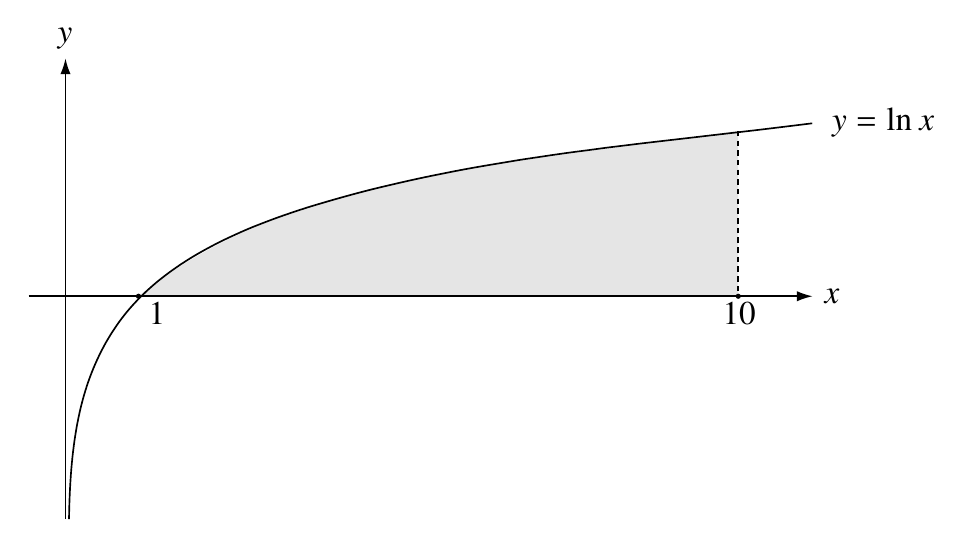
\begin{tikzpicture}[x=0.0127cm,y=-0.0127cm, every node/.style={inner sep=0pt, font=\fontsize{12}{14}\selectfont}]
 \begin{scope}[shift={(25,8)}]
  \fill[black!10] plot[smooth] coordinates {(93,290) (101,283.7) (109,277.7) (117.3,271.8) (125.7,266) (134.1,260.5) (142.7,255.1) (151.5,249.9) (160.2,245) (169.3,240) (178.3,235.4) (187.4,230.9) (196.8,226.5) (206.2,222.3) (215.7,218.2) (225.2,214.3) (235,210.5) (244.6,206.9) (254.5,203.4) (264.4,200.1) (274.4,196.9) (284.5,193.8) (294.6,190.8) (304.7,188) (315.1,185.2) (325.3,182.6) (335.7,180.1) (346,177.7) (356.5,175.3) (367,173.1) (377.5,170.9) (388.2,168.8) (398.8,166.8) (409.4,164.8) (420.2,162.9) (430.8,161.1) (441.6,159.3) (452.4,157.6) (463.2,155.9) (473.9,154.3) (484.9,152.7) (495.8,151.1) (506.6,149.6) (517.6,148.1) (528.4,146.6) (539.4,145.2) (550.4,143.7) (561.4,142.3) (572.4,140.9) (583.6,139.4) (594.5,138) (605.6,136.6) (616.6,135.2) (627.6,133.7) (638.5,132.2) (649.4,130.8) (660.4,129.2) (671.3,127.7) (682.1,126.1) (693,124.5)} -- (693,290) -- cycle;
  \draw[->] (-17,290) -- (767.5,290);
  \draw[->] (20,513) -- (20,52);
  \draw[aux] (693,124.5) -- (693,290);
  \draw plot[smooth] coordinates {(23.5,513) (23.93,496.4) (24.65,480.1) (25.72,464.2) (27.2,448.7) (29.15,433.4) (31.62,418.4) (34.65,403.9) (38.29,389.8) (42.56,376.2) (47.54,363) (53.13,350.4) (59.53,337.9) (66.53,326.2) (74.23,314.9) (82.63,304.2) (91.74,294.1) (101.5,284.5) (112,275.3) (123.5,266.4) (135.2,258.2) (147.8,250.2) (160.8,242.8) (174.3,235.7) (188.2,229.1) (202.6,222.7) (217.1,216.9) (232,211.3) (247.3,206) (262.9,200.9) (278.6,196.2) (294.6,191.6) (310.6,187.2) (326.8,183) (343.1,179.1) (359.5,175.3) (375.8,171.7) (392.2,168.3) (408.8,165) (425.3,161.9) (442,159) (458.7,156.2) (475.7,153.4) (492.4,150.9) (509.2,148.4) (526.3,146) (543.3,143.8) (560.4,141.5) (577.5,139.4) (594.6,137.3) (611.7,135.3) (629,133.3) (646.4,131.3) (663.5,129.3) (680.9,127.3) (698.2,125.3) (715.4,123.3) (732.7,121.2) (749.9,119.1) (767,117)};
  \fill (93,290) circle (2.6) (693,290) circle (2.6);
  \begin{scope}[every node/.append style={anchor=base}]
    \node at (19.5,36) {$y$};
    \node at (111.5,318) {$1$};
    \node at (694,318) {$10$};
    \node[anchor=base west] at (777,297) {$x$};
    \node[anchor=base west] at (786,124) {$y=\ln x$};
  \end{scope}
 \end{scope}
\end{tikzpicture}
\end{document}
